\section{Experimental results}
\label{sec:validation}

In this section we present the results obtained on a special version of the iCub humanoid robot, in which some joints are equipped with joint torque sensors and can provide us with a \emph{ground truth} for the estimation of joint torques and the corresponding identification of the inertial parameters.

\begin{figure}[htb]
\begin{overpic}[width=0.98\textwidth,natwidth=1235,natheight=742]{images/arm3.png}
\put(5,10){FT sensor}
\put(13,13){\vector(1,1){18}}
\put(38,50){Link 1}
\put(43,49){\vector(0,-1){12}}
\put(43,16){Link 2}
\put(47,19){\vector(0,1){8}}
\put(65,45){Link 3}
\put(70,44){\vector(-1,-2){7}}
\put(50,6){Link 4}
\put(57,9){\vector(2,1){19}}
\end{overpic}
\caption{CAD drawing of the seven degree-of-freedom iCub arm used in the experiments. Three out of the four joints (two in the shoulder and one in the elbow) are sensorized with joint level torque sensors. These joints are the one considered in the proposed experiments.}
\label{fig:cadArmMultiBody}
\end{figure}

Experiments were conducted on three joints (pitch and yaw in the shoulder and elbow)\footnote{\href{http://wiki.icub.org/wiki/ICub_joints}{http://wiki.icub.org/wiki/ICub\_joints}} of the iCub left arm (see Fig.~\ref{fig:cadArmMultiBody}). These joints are equipped with joint level torque sensors. Additionally a single F/T sensor is positioned in the middle of the upper arm as represented in Fig.~\ref{fig:cadArmMultiBody}. In the experiment, data from the F/T sensor were used to estimate the associated base parameters. Thanks to the theoretical results presented in the previous sections, these parameters coincides with the one used by the method in the rRNEA to obtain an estimation of the joint torques. These estimations have been compared with direct joint torque measurements, used in this framework as a ground truth. Results are presented in Fig.~\ref{fig:torqueEstimation} where we reported in blue direct joint torque measurements, in red predictions using CAD parameters and in green predictions from the estimation in \cite{Fumagalli2012} supplied with the on-line estimation of the base parameters (presented in Fig.~\ref{fig:paramEstimation}). At the beginning of the simulation estimated parameters are clearly not sufficiently well estimated to predict with sufficient accuracy the joint torques. This condition holds true until the arm starts moving (vertical solid black line in both Fig.~\ref{fig:torqueEstimation} and Fig.~\ref{fig:paramEstimation}).

During the testing trajectories, the end-effector randomly moved in Cartesian space, without any interaction with the environment. Literature on suitable choices of the exciting trajectories is extensive, but such an implementation is out of the scope of the present paper. This simpler choice is also motivated by two factors: first, we need to avoid self-collision of the robot in a simple way; second, we need to generate trajectories similar to those produced during standard operation of the humanoid robot and our goal is to on-line estimate the parameters during standard operations. Joint velocities and accelerations have been estimated using an adaptive-window fitting algorithm \cite{aw2000}. 

%
%%To avoid the problems of causal velocity estimation, the samples are considered for estimation with a delay of half a second, to permit to employ non-causal velocity/acceleration estimation.\\
%To determine the covariance matrix $\boldsymbol\Sigma_n$ of the error of F/T sensor, we analyzed the standard deviation of F/T measurements collected on the still robot. 
%We report the standard deviation on the six axes (the first three components are forces, while the last three are torques): \\
%$$
%\begin{bmatrix} 0.07 & 0.07 & 0.11 & 0.0025 & 0.0030 & 0.0028 \end{bmatrix}
%$$ 
%
%During the test trajectories the torque at the elbow joint was measured with a joint torque sensor, and estimated both with the CAD parameters of the iCub robot and with the parameters identified online. The results are plotted in \ref{fig:torqueEstimation}. It is possible to see how, before the arm starts to move, the torque profile estimated using the identified parameters has no resemblence with the real one, but after the arm start to move the estimation converges to the shape of the measured torque.

\begin{figure}
 \centering
 \includegraphics[width=1.0\textwidth]{images/torque_estimation.pdf}
 % torque_estimation.pdf: 432x293 pixel, 72dpi, 15.24x10.34 cm, bb=0 0 432 293
 \caption{Joint level torques (left part) and errors (right part): measured (black), estimated with CAD parameters (red) and estimated with the procedure in \cite{Fumagalli2012} supplied with identified parameters (green). The vertical solid gray line indicate the movement onset.}
 \label{fig:torqueEstimation}
\end{figure}

\begin{figure*}
 \centering
 \includegraphics[width=1\textwidth]{images/param_identification.pdf}
 % torque_estimation.pdf: 432x293 pixel, 72dpi, 15.24x10.34 cm, bb=0 0 432 293
 \caption{The picture shows the time behavior of the base parameters estimation. The estimation is executed on-line in an iterative fashion. The onset of the movement (vertical solid black line) determines the instant at which the data from the F/T sensor become informative for the estimation problem. Convergence is quite fast and mirrors the behavior of the torques estimation in Fig.~\ref{fig:torqueEstimation}.}
 \label{fig:paramEstimation}
\end{figure*}


% \subsection{Base dynamics prediction}
% In Table \ref{tab:res1}, statistics ($\mu$ for the mean, $\sigma$ for the standard deviation) on the error of prediction of new F/T measurements are reported, obtained on a 10 minute testing trajectory following a 10 minute period of parameter estimation.
% From this results, it is possible to see that the proposed method is able to improve the results obtained with the CAD parameters, 
% without any prior information, using random trajectories which were not optimized for identification. \\

% \subsection{Joint torque predictions}
% We want to use the base parameters to estimate the joint torques. 
% Since the humanoid platform that we used was not equipped with joint torque sensors, 
% we could not compare the joint torque predictions with the ground truth.\\
% Anyway, we carried out a confidence analysis based on the covariance calculation \eqref{eq:quantityCovariance}.
% We plot the standard deviation of the prediction of the four joint torques,
% over 20 minutes, with the inertial parameter estimated online.\\
% The joint torques were predicted using the arm F/T sensor projections combined with the forward torque regressors. \\
% Since the standard deviation of joint torque prediction has a lower magnitude compared
% to the standard deviation of the error of the F/T sensor we can infer that
% the estimation problem is well posed. 



%\begin{figure}[htb]
%\centering
%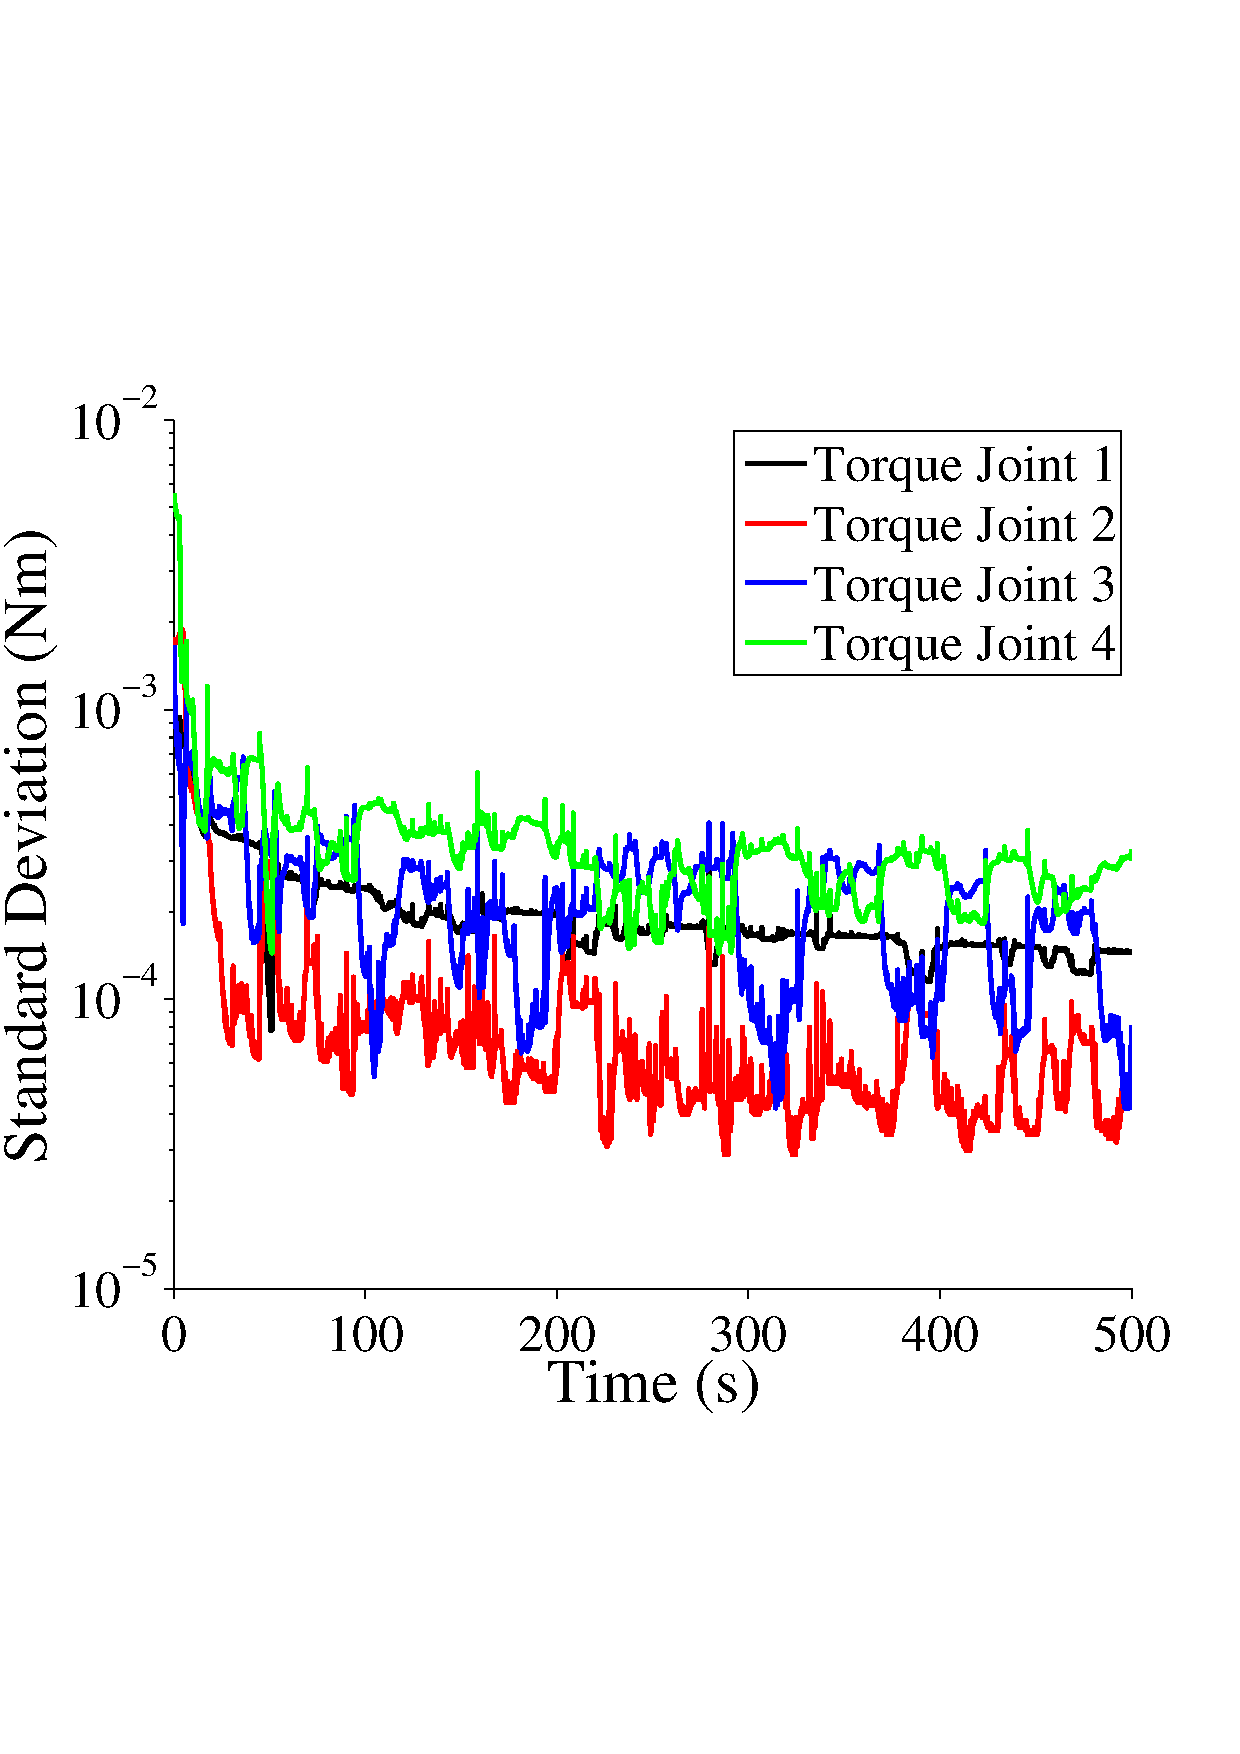
\includegraphics[width=0.4\textwidth]{images/forward_wrench_inc.png}
%\caption{Standard deviation of the four joint torque predictions using online estimated parameters.}
%\label{fig:plot}
%\end{figure}

% 
% \begin{table}[h]
% \caption{Base dynamics prediction errors.}
%     \label{tab:res1}
% \begin{center}
%     \begin{tabular}{ c  c  c  c }
%     \hline
%      &&$\mathbf{F}$(N)&$\boldsymbol\tau$(Nm)\\ [0.5ex] \hline
%      Estimated inertial parameters & $\mu$ & 1.19 & 0.043\\ 
%      CAD inertial parameters & $\mu$ & 1.73 & 0.051\\ 
%      Estimated inertial parameters & $\sigma$ & 0.32 & 0.039\\ 
%      CAD inertial parameters & $\sigma$ & 0.33 & 0.021 \\ [0.5ex] \hline
%     \end{tabular}
% \end{center}
% \end{table}
